\section{Optimization Methods}
\label{sec:method}

\subsection{Gradient Accumulation}

In standard neural network training, we typically divide our data into smaller chunks called mini-batches and process them sequentially. The network generates predictions for each batch, and we compute the loss by comparing these predictions to the actual targets. Afterward, we perform a backward pass to calculate gradients, which are used to adjust the model's weights in the direction of these gradients.

Gradient accumulation alters this last step of the training process. Instead of updating the model's weights after processing each individual batch, we save the gradient values and continue to the next batch, accumulating the new gradients. Weight updates are deferred until the model has processed several batches.

The primary purpose of gradient accumulation is to simulate a larger effective batch size. For instance, imagine you intend to use a batch size of 32 images, but your hardware can handle only up to 8 images without running out of memory. In this scenario, you can work with smaller batches of 8 images and update the weights after every 4 batches by accumulating gradients from each batch in between. To ensure the accumulated gradient remains equivalent to the non-accumulated gradient on a batch of 32 images, you must divide your loss value on each mini-batch of 8 images by 4. Consider a linear model with MSE loss, and mathematically explain why this division step can yield identical results.

\textcolor{red}{
Your answer: Consider a simple linear model \( f(x) = wx + b \), where \( w \) and \( b \) are the model's weight and bias, respectively. The Mean Squared Error (MSE) loss for a set of predictions \( \hat{y} \) and targets \( y \) is given by:
\[
\text{MSE} = \frac{1}{n} \sum_{i=1}^n (\hat{y}_i - y_i)^2
\]
where \( n \) is the number of samples in the batch. The gradient of the loss with respect to the weight \( w \) is computed as follows:
\[
\frac{\partial \text{MSE}}{\partial w} = \frac{2}{n} \sum_{i=1}^n (\hat{y}_i - y_i) \cdot \frac{\partial \hat{y}_i}{\partial w}
\]
Given \( \hat{y}_i = wx_i + b \), where \( \frac{\partial \hat{y}_i}{\partial w} = x_i \), the gradient simplifies to:
\[
\frac{\partial \text{MSE}}{\partial w} = \frac{2}{n} \sum_{i=1}^n (\hat{y}_i - y_i) x_i
\]
Due to hardware limitations, consider using a batch size of 8 and accumulating gradients over 4 such mini-batches to simulate an effective batch size of 32. The gradient for each mini-batch of 8 samples is:
\[
\frac{\partial \text{MSE}_{\text{mini}}}{\partial w} = \frac{2}{8} \sum_{i=1}^8 (\hat{y}_i - y_i) x_i
\]
After processing 4 mini-batches, the accumulated gradient becomes:
\[
\text{Accumulated gradient} = 4 \times \frac{2}{8} \sum_{\text{all } 32 \text{ samples}} (\hat{y}_i - y_i) x_i = \frac{2}{2} \sum_{\text{all } 32 \text{ samples}} (\hat{y}_i - y_i) x_i
\]
If we divide the loss of each mini-batch by 4, the gradient for each batch becomes:
\[
\frac{\partial \text{MSE}_{\text{mini}}}{\partial w} = \frac{1}{4} \cdot \frac{2}{8} \sum_{i=1}^8 (\hat{y}_i - y_i) x_i
\]
Thus, accumulating this gradient over 4 batches yields:
\[
\text{Accumulated gradient} = \frac{1}{4} \cdot 4 \times \frac{2}{8} \sum_{\text{all } 32 \text{ samples}} (\hat{y}_i - y_i) x_i = \frac{2}{32} \sum_{\text{all } 32 \text{ samples}} (\hat{y}_i - y_i) x_i
\]
This adjustment ensures that the accumulated gradient matches the gradient computed for a single batch of 32 samples, thereby maintaining consistency in learning updates.
This shows that dividing the MSE loss by the number of mini-batches (4 in this case) ensures the accumulated gradient matches the gradient computed for a single batch of 32 samples.
}

However, it's important to note that gradient accumulation may not always yield identical results, especially for deep neural network architectures that employ batch-wise regularization methods like batch normalization. Batch normalization relies on statistics calculated within each batch, and when you accumulate gradients, these statistics may not be consistent. Mathematically explain the batch normalization layer behavior and why gradient accumulation yields non-identical results in this case.

\textcolor{red}{
Your answer: Batch normalization involves normalizing the input layer by adjusting and scaling the activations. Mathematically, for a given feature in a batch, batch normalization is defined as:
\[
\text{BN}(x_i) = \gamma \left(\frac{x_i - \mu_B}{\sqrt{\sigma_B^2 + \epsilon}}\right) + \beta
\]
where \( x_i \) are the inputs to the layer, \( \mu_B \) is the mean of the batch, \( \sigma_B^2 \) is the variance of the batch, \( \gamma \) and \( \beta \) are parameters to be learned, and \( \epsilon \) is a small constant added for numerical stability.
\newline
The key point in batch normalization is that it relies on the mean (\( \mu_B \)) and variance (\( \sigma_B^2 \)) computed from the current batch. When using gradient accumulation, each mini-batch contributes to the accumulated gradient, but the batch normalization statistics (\( \mu_B \) and \( \sigma_B^2 \)) are recalculated for each mini-batch. This means the normalization is performed using different means and variances across these batches.
Therefore, even though gradients are accumulated, the differing batch statistics lead to discrepancies in the normalized inputs each time, potentially affecting the learning dynamics. Consequently, the updates computed through gradient accumulation with batch normalization may not perfectly simulate the updates that would be computed in a single larger batch.
}

\subsection{Gradient Checkpointing}

Gradient checkpointing is another memory-saving technique that strikes a balance between memory and computation during neural network training. While it's well understood that storing all activations and intermediate results from the forward pass is essential for performing backward propagation, this process can lead to a significant increase in memory usage, often referred to as the "memory blow-up" problem. When monitoring memory consumption during model training, you'll notice that it gradually accumulates and reaches its peak after completing the forward pass. Explain why model inference does not have such ``memory blow-up" problem.

\textcolor{red}{
Your answer: Model inference doesn't experience the "memory blow-up" problem seen in training primarily because it only involves the forward pass of the neural network. During inference, the network computes output predictions from given inputs, using the learned weights and biases. Crucially, it does not require the storage of intermediate activations needed for backpropagation, as no learning or adjustment of weights occurs. This means the memory footprint is much smaller during inference compared to training, where memory needs to accommodate both the activations for computing gradients and the gradients themselves.
}

Instead of retaining all activations and intermediate results in memory throughout the forward pass, gradient checkpointing offers an alternative approach. It strategically selects checkpoints within the network where memory efficiency takes precedence over computation time. When the algorithm encounters these checkpoints during the subsequent backward pass, it does not rely on stored activations because they were not stored in memory in the first place. Instead, it recalculates them by re-executing the forward pass up to the specific checkpoint.

To optimize memory usage and forward computation steps using gradient checkpointing in a feed-forward neural network composed of $n$ layers, let's consider two strategies: Imagine a simple feed-forward neural network with $n$ layers, each generating activations of the same size. Upon completing the forward pass, the algorithm retains all activations, resulting in an $O(n)$ memory requirement for this network. In other words, it consumes $n$ units of memory. In terms of computation, the forward pass requires $O(n)$ steps, assuming that each layer requires 1 unit of computation.

Now, the question revolves around determining the optimal placement of checkpoints to strike a balance between memory and computation. A poor strategy would be discarding all activations during the forward pass and recomputing them later when needed. Conversely, a more general and optimal strategy suggests discarding activations every $\sqrt{n}$ steps. What are the memory requirement and forward computation steps for the two strategies in big O notation? Check this medium post \cite{checkpointing} for more illustrations.

\textcolor{red}{
Your answer: The two strategies in gradient checkpointing for managing memory and computation in a feed-forward neural network with \( n \) layers are summarized below in terms of their big \( O \) notation for memory and computation requirements:
\textbf{Strategy 1 (Discarding all activations during forward pass):} The memory requirement is \( O(1) \), as only the current activation is stored at any time, with all others discarded and recalculated as needed. The forward computation steps are \( O(n^2) \), since every time a gradient is needed for a layer during the backward pass, the forward computations for all preceding layers up to that point must be redone, leading to a quadratic increase in computational steps.
\textbf{Strategy 2 (Checkpointing every \( \sqrt{n} \) steps):} The memory requirement is \( O(\sqrt{n}) \), with checkpoints saved after every \( \sqrt{n} \) layers, resulting in approximately \( \sqrt{n} \) checkpoints stored. The forward computation steps are \( O(n \sqrt{n}) \), as for each of the \( n \) layers, if its activation needs to be recomputed during the backward pass, it involves re-executing the forward pass from the nearest preceding checkpoint, averaging out to \( \sqrt{n} \) recomputation steps per layer.
}

In practical scenarios, neural networks often feature layers with varying activation sizes, and the computational complexity of each layer's forward pass can differ significantly. Furthermore, the forward graph of these networks may not adhere to a strictly sequential pattern. Consequently, the task of strategically placing checkpoints to optimize memory usage and computation steps remains an active area of research and attention. 


\subsection{Low-Rank Adaptation (LoRA)}

Parameter-efficient Fine-tuning (PEFT) is a technique in NLP that enhances the performance of pre-trained language models on specific tasks. It freezes most of the pre-trained model's parameters and only fine-tunes a subset of layers, reducing computational and memory demands and training time, while retaining a good performance as possible. The idea of reducing the number of trainable parameters has its roots in transfer learning within computer vision tasks, where traditionally, only the final fully connected layer was updated.

Before we dive into the technical aspect of Low-Rank Adaptation (LoRA), one must revisit the transformer architecture and understand the mechanism of self-attention. In addition, LoRA uses the concept of truncated Singular Value Decomposition (SVD). Please study and understand the concepts of SVD and truncated SVD. Answer the following questions:

\begin{enumerate}
    \item What is matrix rank?
    \item What are three decomposed matrices by SVD? 
    \item $U$ and $V$ are orthogonal matrices. Why does it imply $UU^T=I, VV^T=I$?
    \item If a matrix $W \in {R ^{n \times n}}$ is full rank, what is its rank?
    \item Suppose a full rank matrix $W \in {R ^{n \times n}}$ represents an image. After we apply SVD to this matrix, we modify the singular matrix by only keeping its top-$k$ singular values and discarding the rest (i.e., set the rest of the singular values to zero). Then, we reconstruct the image by multiplying U, modified S, and V. What would the reconstructed image look like? What if you increase the values of $k$ (i.e., keep more singular values)?
    \item If a matrix $W \in {R ^{n \times n}}$ is low rank, what does its singular matrix look like?
    \item If the top-$k$ singular values of a matrix $W \in {R ^{n \times n}}$ are large, and the rest are near zero, this matrix $W$ exhibits low-rank or near-low-rank behavior. Can you represent $W$ by two low-rank matrices, $A$ and $B$? If so, what are those two matrices' expressions in terms of $U$, $S$, and $V$? Do you think those two matrices are a good approximation of $W$ (i.e., $W \approx AB$)?
    \item The above operation is called truncated SVD. Under what situation do you think truncated SVD fails to make a good approximation? Think about the singular matrix.
\end{enumerate}

\textcolor{red}{
Your answer: \newline
1. The matrix rank is a measurement of dimension of the vector space spanned by its rows or columns. It tells how much information contained in the matrix and how many dimensions can be described by rows or columns.
\newline
2. Let \( A \) be a sample matrix. The first matrix is \( U \), which is an \( m \times m \) orthogonal matrix. The columns of \( U \) are the eigenvectors of \( A A^T \). The second matrix is \( \Sigma \), which is an \( m \times n \) diagonal matrix containing the singular values of \( A \). The third matrix is
\newline
3. As \( U \) is an orthogonal matrix, the columns of \( U \) are orthonormal. Thus, each element \( u_{ij} \) in matrix \( U \) is the dot product of column \( i \) of \( U \) with column \( j \) of \( U \). Since the columns are orthonormal, the dot product of any column with itself should be 1 and the dot product of different columns should be 0. Therefore, \( UU^T = I \). Similarly, for \( V^T \), changes pertain to the dot product of row \( i \) of \( V^T \) with row \( j \) of \( V^T \). The diagonal entries will be the dot product of each column with itself, which is 1, and the off-diagonal entries will be zero. Therefore, \( V^TV = I \).
\newline
4. Full rank means \( W \) is an \( n \times n \) matrix and all \( n \) columns are linearly independent, so the rank is \( n \).
\newline
5. Retaining only top-\( k \) singular values in \( \Sigma \) means lowering the singular values, causing the reconstructed image to lose some details. If we keep more singular values, as \( k \) increases, it will improve the fidelity. The image will become sharper and has more details in it. Overall, smaller \( k \) compresses the image while larger \( k \) emphasizes fidelity to the original image.
\newline
6. Its singular matrix will have sparse non-zero entries which means most singular values will be zero. The singular values in \( \Sigma \) are arranged in descending order which means the largest singular values will appear first on the diagonal, followed by smaller values and then zeros.
\newline
7. First, set \( U_k \) as the new \( U \) containing the first \( k \) columns, \( \Sigma_k \) as the new \( \Sigma \) containing the top left \( k \times k \) blocks of \( \Sigma \) with the largest \( k \) singular values, and \( V_k \) as the new \( V \) containing the first \( k \) columns. Define \( A = U_k \Sigma_k^{1/2} \) and \( B = \Sigma_k^{1/2} V_k^T \). Now we can compute \( AB = U_k \Sigma_k^{1/2} \Sigma_k^{1/2} V_k^T = U_k \Sigma_k V_k^T \), which is the approximation to \( W \) in terms of the Frobenius norm. This is a good approximation if \( k \) is large enough.
\newline
8. It is a good approximation method. However, if the lower singular values contain a significant amount of information, it could fail as there might be too much information relevant to the data structure. The omission can lead to substantial loss of information.
}


Now, you are equipped with the knowledge to understand LoRA. As one of the most effective PEFT techniques, proposed by Edward Hu et al. in 2021 \cite{hu2021lora}, the success of LoRA is based on an important observation that both pre-trained weights and change of weights during fine-tuning for LLMs are low-rank matrices.

To illustrate this, consider representing the final optimal weights after fine-tuning as $W^* = W_0 + \Delta W$, where $W_0 \in {R}^{n \times n}$ represents the pre-trained weights, and $\Delta W \in {R}^{n \times n}$ captures the weight changes during fine-tuning. Notably, $\Delta W$ can be approximated as the product of two matrices, $AB$, with $A \in {R}^{n \times r}$ and $B \in {R}^{r \times n}$. This implies that during fine-tuning, we don't have to update the whole matrix $W_0$. Instead, we modify the forward pass in the layer, changing it from $y = xW_0$ to $y= xW_0 + xAB = x(W_0 + AB)$, as depicted in Figure \ref{fig:lora}. We freeze $W_0$ and only update $A$ and $B$. Notice that since $r << n$, the total number of parameters of $A$ and $B$ is much smaller than that of $W_0$. To make the modified forward pass identical to the original one at the beginning of fine-tuning, $A$ is randomly initialized in Gaussian distribution, and $B$ is initially set to 0, so $AB=0$. 

\begin{figure}[h]
    \centering
    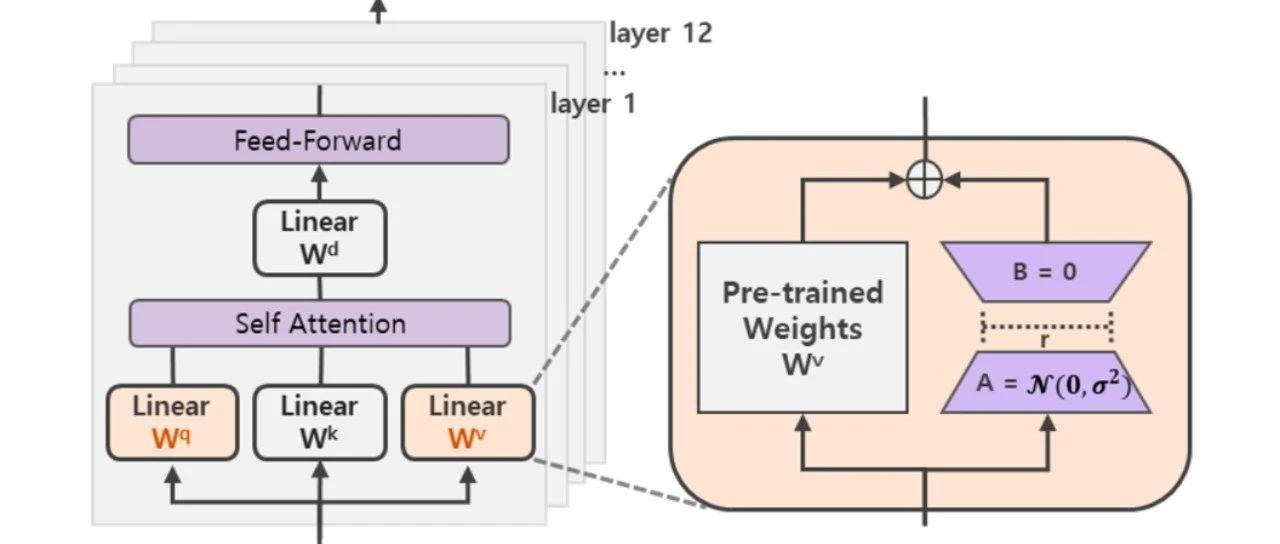
\includegraphics[width=\textwidth]{figures/lora.jpeg}
    \caption{LoRA}
    \label{fig:lora}
\end{figure}

Technically, we can insert $A$ and $B$ into any layers, such as the query, key, value, output projection layers, or the FFN layers in each attention block. However, the paper suggests that applying LoRA only to query and value projection layers can yield performance comparable to full parameter fine-tuning. The hyperparameter $r$ typically takes on small values within the range of 4 to 32. 
By inserting $A$ and $B$ into specific layers and keeping the rest of the pre-trained weights frozen, LoRA achieves a substantial reduction in the total number of trainable parameters. For $r=8$, the percentage of parameters that are subject to training accounts for less than $1 \%$ of the overall parameters in a typical LM. This remarkable reduction in the number of trainable parameters is a key factor in the efficiency of LoRA as a PEFT technique.

It seems like applying LoRA would add more parameters to the model, thus increasing forward pass costs and inference latency. How does LoRA paper overcome this drawback?

\textcolor{red}{
Your answer: In this paper, we introduce a low-rank structure, as \( A \) and \( B \) are low-rank matrices, they introduce significantly fewer parameters than a full matrix. This reduction allows for an increase in parameter count while reducing computational costs. Another method involves updating \( A \) and \( B \), capitalizing on the parameter efficiency. \textit{LoRA} updates a small fraction of the total number of parameters, which can yield performance comparable to full parameter fine-tuning. By updating the dense matrix \( W_0 \), the multiplication of \( A \times B \) can be optimized during the forward and backward pass. Moreover, \textit{LoRA}'s implementation can leverage efficient linear algebra operations, which are optimized on the hardware, thereby keeping the computational cost low.
}

\subsection{Mixed Precision Training}
Mixed precision training \cite{micikevicius2018mixed} is a technique used in large neural network training that combines the use of both 16-bit and 32-bit floating-point representations for different parts of the training process. This approach leverages the advantages of lower precision (16-bit) for some computations while still using higher precision (32-bit) where necessary. 

As illustrated in Figure \ref{fig:amp}, during the forward pass, the model converts the FP32 weights to FP16 and computes FP16 activations, and in the backward pass, both activation gradients and weight gradients are calculated in FP16. Subsequently, the FP32 master copy of weights is updated with the FP16 weight gradients. The authors also claim that some operations should be read and written in FP16 but perform arithmetic in FP32 to maintain model accuracy. Read the paper and answer why we need an FP32 master copy of weights and why we need to scale up the loss.

\textcolor{red}{
Your answer: An FP32 master copy of weights in mixed precision training is crucial to preserve small gradient values that would otherwise become zero in FP16 due to its limited range and precision. This ensures that all updates, no matter how small, contribute to the learning process. Loss scaling is used to prevent small-magnitude gradients from underflowing to zero in FP16 by temporarily increasing their size, allowing them to be represented in the reduced precision format during back-propagation. Afterward, the gradients are scaled back to their original size before updating the weights.
}

FP16 operations offer significant speed advantages over FP32 operations, especially on modern GPUs equipped with NVIDIA's Volta and Ampere architectures. These architectures include dedicated hardware, known as Tensor Cores, designed to accelerate FP16 multiplication and accumulation into either FP16 or FP32 outputs. Thus, it is clear that mixed precision training can reduce computation time by utilizing FP16 computation units. In terms of memory consumption, according to the paper:

``Even though maintaining an additional copy of weights increases the memory requirements for the weights by 50\% compared with single precision training, impact on overall memory usage is much smaller. For training memory consumption is dominated by activations, due to larger batch sizes and activations of each layer being saved for reuse in the back-propagation pass. Since activations are also stored in half-precision format, the overall memory consumption for training deep neural networks is roughly halved. "

Do you think this statement still holds for LLM fine-tuning?

\textcolor{red}{
Your answer: Yes, the statement about mixed precision training reducing overall memory consumption likely still holds for fine-tuning large language models (LLMs). This is because activations, which are stored for use in the backward pass, typically use the most memory during training. Since activations can be stored in FP16 format, this significantly reduces memory usage. Even though maintaining an FP32 copy of the weights increases memory requirements for the weights by 50\% compared to FP32 alone, the reduction in memory from using FP16 for activations generally results in a net decrease in overall memory consumption. Additionally, the use of FP16 allows for leveraging specialized GPU hardware like Tensor Cores for faster computations.
}

\begin{figure}[h]
    \centering
    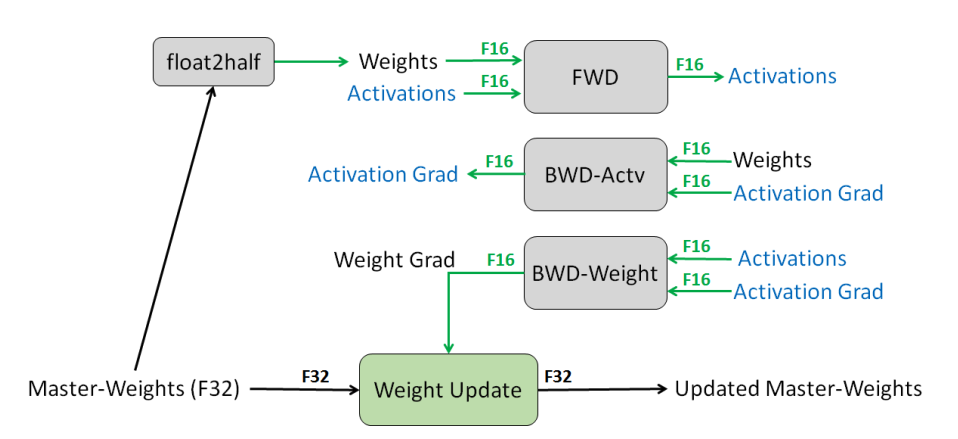
\includegraphics[width=\textwidth]{figures/amp.png}
    \caption{Mixed precision training}
    \label{fig:amp}
\end{figure}